\section*{15/07/2022 --- Controle por Lyapunov}
\markboth{Controle por Lyapunov}{15/07/2022}
\noindent\textbf{\sffamily Exercício 1.}
	Encontre um controle $u$ de Lyapunov que estabilize o pêndulo sem atrito,
	%
	\[
	    \ddot{x} = -\sin x + u,
	\] 
	%
	em $x=\pi/2$. \\

\noindent{\textbf{{\sffamily Exercício 2.}}
	Estabilize o sistema anterior no ponto $x=\pi/4$ com um novo controle mais inteligente.\\
	
\noindent{\textbf{{\sffamily Exercício 3.}}
	Proponha um sistema de controle por Lyapunov para o sistema dinâmico abaixo.
	%
	\[
		\frac{d^2\theta}{d\theta^2} = -2\theta 
		                              -4\frac{d\theta}{dt} 
		                              +\left(\frac{d\theta}{dt}\right)^{\!3}
		                              +u
	\]
	%
\noindent{\textbf{{\sffamily Exercício 4.}}
	Repita o exercício anterior trocando a parcela $-2\theta$ na EDO por $-2\theta^3$. \\
	
\noindent{\textbf{{\sffamily Exercício 5.}}
	Repita o exercício 3 trocando a parcela $-2\theta$ na EDO por $-2\theta^2$. \\
\rule{\textwidth}{0.5pt}\\

\noindent{\textbf{{\sffamily Exercício 1 --- solução.}} \\
	Pensando matematicamente, procuramos um ``equilíbrio deslocado", em comparação com os clássicos equilíbrios na origem.
	Pondo dessa maneira, faz sentido tentar $H$ de Lyapunov dada por 
	%
	\[
		H(x) = \frac{\dot{x}^2}{2} + 
		       \frac{\e}{2}\left(x-\frac{\pi}{2}\right)^2.
	\]
	%
	$\e>0$ é posto para garantir a positividade definida da função.
	Derivando, vem
	%
	\begin{align*}
		\dot{H} &= \dot{x}\ddot{x} + \e\left(x-\frac{\pi}{2}\right)\dot{x} \\
		        &= \dot{x}(\ddot{x} + \e\left(x-\frac{\pi}{2}\right)) \\
		        &= \dot{x}(-\sin x + \e\left(x-\frac{\pi}{2}\right) + u).
	\end{align*}
	%
	Logo, uma lei de controle que satisfaz $\dot{H}\leq 0$ é 
	$u = \sin x -\alpha\dot{x} - \e\left(x-\frac{\pi}{2}\right)$, $\alpha>0$. \\
	
\noindent{\textbf{{\sffamily Exercício 2 --- solução.}} \\
	Trocar $\pi/2$ por $\pi/4$ na $H$ acima resultaria no controle
	$u = \sin x -\alpha\dot{x} - \e\left(x-\frac{\pi}{4}\right)$, $\alpha>0$.
	
	O problema com tal $u$ é que pequenos distúrbios no ponto de equilíbrio são amplificados pelo seno antes de serem efetivamente reduzidos pelo ``atrito" $-\e x$.
	Esse comportamento é precisamente oposto ao da função cosseno, e por causa disso o objetivo será trocar na lei de controle original o seno pelo cosseno.
	
	Realizando a substituição, e a partir daí reconstruindo $H$, chegamos à seguinte expressão:
	%
	\begin{align*}
		\dot{H} &= \dot{x}(u-\cos x +\e\left(x-\frac{\pi}{4}\right)) \\ 
		        &= \dot{x} (\ddot{x} + \sin x - \cos x 
		                   + \e\left(x-\frac{\pi}{4}\right)) \\
		        &= \dot{x}\sqrt{2}\sin\left(x-\frac{\pi}{4}\right) +
		           \dot{x}\e\left(x-\frac{\pi}{4}\right) +
		           \dot{x}\ddot{x} \\
		\implies
		H(\theta) &= \sqrt{2}(c_1 - \cos\left(x-\frac{\pi}{4}\right)) +
		             \frac{\e}{2}\left(x-\frac{\pi}{4}\right)^2 +
		             \frac{\dot{x}^2}{2}.
	\end{align*}
	%
	Escolhendo $c_1=1$, $H$ acima se torna positiva definida com derivada $\leq0$ através do controle proposto, e o problema está fechado. \\
	%
	\begin{figure}[H]\centering
		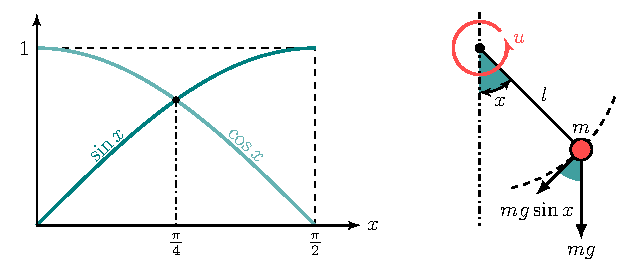
\includegraphics{sen vs cos.pdf}
		\caption{%
			Quando $x=\pi/4+\delta$, $u$ com $\sin x$ aumenta, distanciando o pêndulo do equilíbrio, enquanto $u$ com $\cos x$ diminui, facilitando a volta ao equilíbrio pela força peso.
			Quando $x=\pi/4-\delta$, $u$ com $\cos x$ aumenta para compensar a força peso, enquanto $\sin x$ relaxa, novamente distanciando o pêndulo do equilíbrio.
		}
	\end{figure}
	
\noindent{\textbf{{\sffamily Exercício 3 --- solução.}}\\
	Aqui vale tomar $H$ como a consagrada combinação linear entre $\theta$ e suas derivadas. Por exemplo, considere
	%
	\[
		H(\theta) = \frac{\dot{\theta}^2}{2} + 2\frac{\theta^2}{2}.
	\]
	%
	Perceba que a função acima é positiva definida. 
	Derivando-a no tempo, temos
	%
	\begin{align*}
		\dot{H} &= \dot{\theta}\ddot{\theta} + 2\theta\dot{\theta} \\
		        &= \dot{\theta}(\ddot{\theta} + 2\theta) \\
		        &= \dot{\theta}(-4\dot{\theta} + \dot{\theta}^3 + u),
	\end{align*}
	%
	de maneira que, para obter $\dot{H} \leq 0$, podemos escolher por exemplo 
	$u = -\dot{\theta}^3$. 
	
	De fato, tal $u$ nos leva a $\dot{H} = -4\dot{\theta}^2 \leq 0$. \\
	
\noindent{\textbf{{\sffamily Exercício 4 --- solução.}}\\
	Fisicamente, tanto $-2\theta$ quanto $-2\theta^3$ podem ser interpretados como coeficientes de atrito à variação de $\theta$, de forma que o novo sistema continua estável como o original. 
	
	Entretanto, tomar $H$ como no exercício anterior levaria a uma lei de controle talvez demasiadamente carregada, e assim o desafio aqui será definir $H$ que dê o mesmo $u$ anterior. 
	Conseguimos isso incluindo na função de Lyapunov a integral (em $\theta$) da parcela nova:
	%
	\begin{align*}
		H(\theta) = \frac{\dot{\theta}^2}{2} + 2\frac{\theta^4}{4} 
		\implies
		\dot{H} &= \dot{\theta}\ddot{\theta} + 2\theta^3\dot{\theta} \\
		        &= \dot{\theta}(\ddot{\theta} + 2\theta^3) \\
		        &= \dot{\theta}(-4\dot{\theta} + \dot{\theta}^3 + u) 
		        \leq 0
		\implies u = -\dot{\theta}^3,
	\end{align*}
	%
	como desejávamos. \\

\noindent{\textbf{{\sffamily Exercício 5 --- solução.}}\\
	Ao contrário dos problemas anteriores, a nova parcela não pode mais ser entendida como um atrito, e sua integral em $\theta$ não é positiva definida. 
	Para nos livrarmos desse empecilho, tentativamente tomamos
	%
	\[
		H(\theta) = \frac{\dot{\theta}^2}{2} +
		            2\frac{\theta^2|\theta|}{3},
	\]
	%
	de forma que, para $\theta\geq0$,
	%
	\begin{flalign*}
		\dot{H} &= \dot{\theta}\ddot{\theta} + 2\theta^2\dot{\theta} & \\
		        &= \dot{\theta}(\ddot{\theta} + 2\theta^2) \\
		        &= \dot{\theta}(-4\dot{\theta} + \dot{\theta}^3 + u) 
		        \leq 0
		\implies
		u = -\dot{\theta}^3,
	\end{flalign*}
	%
	e para $\theta<0$,
	%
	\begin{flalign*}
		\dot{H} &= \dot{\theta}\ddot{\theta} - 2\theta^2\dot{\theta} & \\
		        &= \dot{\theta}(\ddot{\theta} - 2\theta^2) \\
		        &= \dot{\theta}(-4\dot{\theta} - 4\theta^2 + \dot{\theta}^3 + u) 
		        \leq 0
		\implies
		u = -\dot{\theta}^3 + 4\theta^2.
	\end{flalign*}
	%
	Unindo as leis de controle numa única equação, ficamos com 
	$u(t) = -\dot{\theta}^3 + 2\theta(\theta - |\theta|)$.
	 